% !TEX TS-program = pdflatex
% !TEX encoding = UTF-8 Unicode

% This is a simple template for a LaTeX document using the "article" class.
% See "book", "report", "letter" for other types of document.

\documentclass[11pt]{article} % use larger type; default would be 10pt

\usepackage[utf8]{inputenc} % set input encoding (not needed with XeLaTeX)

%%% Examples of Article customizations
% These packages are optional, depending whether you want the features they provide.
% See the LaTeX Companion or other references for full information.

%%% PAGE DIMENSIONS
\usepackage{geometry} % to change the page dimensions
\geometry{a4paper} % or letterpaper (US) or a5paper or....
% \geometry{margin=2in} % for example, change the margins to 2 inches all round
% \geometry{landscape} % set up the page for landscape
%   read geometry.pdf for detailed page layout information

\usepackage{graphicx} % support the \includegraphics command and options

% \usepackage[parfill]{parskip} % Activate to begin paragraphs with an empty line rather than an indent

%%% PACKAGES
\usepackage{booktabs} % for much better looking tables
\usepackage{array} % for better arrays (eg matrices) in maths
\usepackage{paralist} % very flexible & customisable lists (eg. enumerate/itemize, etc.)
\usepackage{verbatim} % adds environment for commenting out blocks of text & for better verbatim
\usepackage{subfig} % make it possible to include more than one captioned figure/table in a single float
\usepackage{amsmath}
\usepackage{mathtools}
\usepackage{lmodern}
\usepackage{graphicx}
\usepackage{listings}
\usepackage{color}
\usepackage{float}
\usepackage{amssymb}
% These packages are all incorporated in the memoir class to one degree or another...

%%% HEADERS & FOOTERS
\usepackage{fancyhdr} % This should be set AFTER setting up the page geometry
\pagestyle{fancy} % options: empty , plain , fancy
\renewcommand{\headrulewidth}{0pt} % customise the layout...
\lhead{}\chead{}\rhead{}
\lfoot{}\cfoot{\thepage}\rfoot{}

%%% SECTION TITLE APPEARANCE
\usepackage{sectsty}
\allsectionsfont{\sffamily\mdseries\upshape} % (See the fntguide.pdf for font help)
% (This matches ConTeXt defaults)

%%% ToC (table of contents) APPEARANCE
\usepackage[nottoc,notlof,notlot]{tocbibind} % Put the bibliography in the ToC
\usepackage[titles,subfigure]{tocloft} % Alter the style of the Table of Contents
\renewcommand{\cftsecfont}{\rmfamily\mdseries\upshape}
\renewcommand{\cftsecpagefont}{\rmfamily\mdseries\upshape} % No bold!

%%% MY COMMANDS
\renewcommand{\vec}[1]{\underline{#1}}
\DeclarePairedDelimiter{\norm}{\lVert}{\rVert}
\newcommand*{\addheight}[2][.5ex]{%
  \raisebox{0pt}[\dimexpr\height+(#1)\relax]{#2}%
}

%%% SET CODING LANGUAGE
\lstset{frame=tb,
  language=Matlab,
  aboveskip=3mm,
  belowskip=3mm,
  showstringspaces=false,
  columns=flexible,
  basicstyle={\small\ttfamily},
  numbers=none,
  numberstyle=\tiny\color{gray},
  keywordstyle=\color{blue},
  commentstyle=\color{dkgreen},
  stringstyle=\color{mauve},
  breaklines=true,
  breakatwhitespace=true,
  tabsize=3
}

%%% END Article customizations

%%% The "real" document content comes below...

\title{Object Detection within Cluttered Images with PCA versus Sparse Matrix}
\author{Patrick Talley
  \vspace{0.5in} \\
  under the direction of \\
  Prof. Gesualdo Scutari \\
  Purdue University \\
  \vspace{1in}}
\date{} % Activate to display a given date or no date (if empty),
         % otherwise the current date is printed

\begin{document}
\maketitle
%\pagebreak
\begin{abstract}
Finding objects within an image is a challenging task. There is often clutter, and understanding the difference between objects can be challenging. In this paper
a comparison between Principal Componenet Analysis, PCA, with eigenvectors, and Low Rank + Sparse Matrix representation were compared. This was done on fishing
photos from The Nature Conservancy with the goal of singling out the fish within the image. What was found was that the Sparse Matrix was able to capture the fish's
features much more consistently than PCA.
\end{abstract}

\pagebreak

\tableofcontents

\pagebreak
\section{Introduction}
The topic is trying to find an object given a dictionary using PCA and sliding window.
The image is very noisy, and the object has many different forms.
This topic specifically attempts to address a challenge proposed by The Nature Consevancy,
where they wish to identify species caught by fishing boats to reallocate human capital for enforcement.
In order to tackle to challenge, and find the fish, a basis of fish was found by using 100 images cropped to only contain the fish.
Once this basis was found, a sliding window going through a 20x20 block of the tested image was then tested against this basis.
If the projection was within a threshold then the block will be treated as containing the fish. This creates a sparse representation of the image useful for further analysis.
The reason that this approach was used was specifically to attempt to detect the difference between a fish and the background.  \\
A second option to find this was by the creation of a sparse matrix, and a low rank matrix. While there exists a large amount of clutter, PCA often
fails due to corruption, and this approach is more robust. A sparse matrix containing the figures of the fish, and a low rank matrix containing the boat and ocean will
be created. A comparison of these approaches for the type of problem as far as containment of the fish, and number of non-zeros of the resulting matrices.

\section{Problem Formulation}
\subsection{PCA with Sliding Window}
The main issue that arises when attempting to use principal componenet analysis is that the picture is very noisy
and as such it will have difficulties differentiating between the correct object and others. PCA works by
creation of a basis using k eigen vectors. \\
Consider a set of n fish images $X=\{x_1,x_2,...,x_n\}$, where each $x_i$ represents a vector of the fish image.\\
Let $\bar{\vec{x}}$ by the average fish among $X$ then normalize the fish such that $\tilde{X} = X- \bar{\vec{x}}$ \\
Then project the faces. Because $X$ is such a large matrix in order to create the eigenvectors singular value decomposition will be used.\\
\[\tilde{X}^{T}\tilde{X} = V \Sigma ^2 V^{T} \]
Let $V_k$ be the fist $k$ vectors in $V$. \\
Then from $V^{T}V=I$
\[ \tilde{X} \vec{v_1} = U \Sigma V^{T} v_{1} = U \Sigma \begin{bmatrix}1 \\0 \\...\\ 0 \end{bmatrix} = U\begin{bmatrix}\sigma \\ 0 \\... \\0\end{bmatrix} = \sigma_1 u_1 \]
\[u_1 = \frac{\tilde{u_1}}{\norm{\tilde{u_1}}} \]
Now we have a matrix $A = $ first k elements of $U$ normalized. Create a projection space $P_{x_1} = A^{T}*\tilde{x_1}$ for all $\tilde{x_i}\in\tilde{X}$
\\
When given an image to test against $Y$ it will be broken up into 20x20 pixel squares, $S$. This sliding square will cycle through the image and project into the space.
\[P_y = A^{T}*\vec{s} \]
Then it will be tested agains $P_x$ to determine if this square is a fish or not.
\[\bar{F} = \frac{1}{n} \sum_{i=1}^n \norm{P_y - P_{x_i}} \]
If $\bar{F}\leq \phi$ where $\phi$ is the threshold, then it will be included in the image.

\subsection{Low Rank Approximation}
Given an image $Y$ there arises a need to create a matrix $A$ and a matrix $E$, where $A$ is the lowest rank that agrees with the data, and $E$ is some sparse matrix.
A natural extension of this is to create the following formulation
\[min \ rank(A) + \lambda \norm{E}_0 \ subj A+E=Y\]
However, the $l_0$ and the rank is non-convex. So to approximate this minimization problem the nuclear norm, and $l_1$ norm are used.
\[min \ \norm{A}_{*} + \lambda \norm{E}_{0} \ subj A + E =Y \]
The $l_1$ norm is the convex envelope of the $l_0$ norm, that is it is the best approximation while remaining convex. This program is semidefinite and can be solved in polynomial time.
In order to determine $\lambda$ a non-adaptive weight factor is used. For this instance it is $\frac{1}{\sqrt{max\{n,m\}}}$ where $n,m$ are the dimensions of $Y$.
\[ \therefore (A_{0} ,E_{0}) = argmin \ \norm{A}_{*} + \lambda \norm{E}_{1} \ subj A+E = Y\]
And the matrix we want is the sparse matrix $E$ which should contain the fish within the image.

\section{Main Contribution}
To perform PCA for this image, it was done through the creation of an eigenspace which to project a vector into. In order to try and match and object, a
sliding window technique was used. The reason that this attempting to work around the noise and similarity to other objects within with image to the fish.
\\
This was tested against a sparse representation in order to determine which of the two could correctly identify this image among the noise. Given the
need to use these detection algorithms within a robust range of cases having alternatives to the requirements of eigenfaces. The sparse matrix
does not require well constructed test cases to be used. This makes it attractive to be put in place more applications.

\section{Numerical Results}
\section{PCA}
A basis using cropped fish were used from a variety of images. The dataset was provided by The Nature Conservancy. To simplify the test cases
they were resized from the original resolution of 1280x720 to 240x240. The image was also altered to greyscale for simplicity.
\begin{figure}[h]
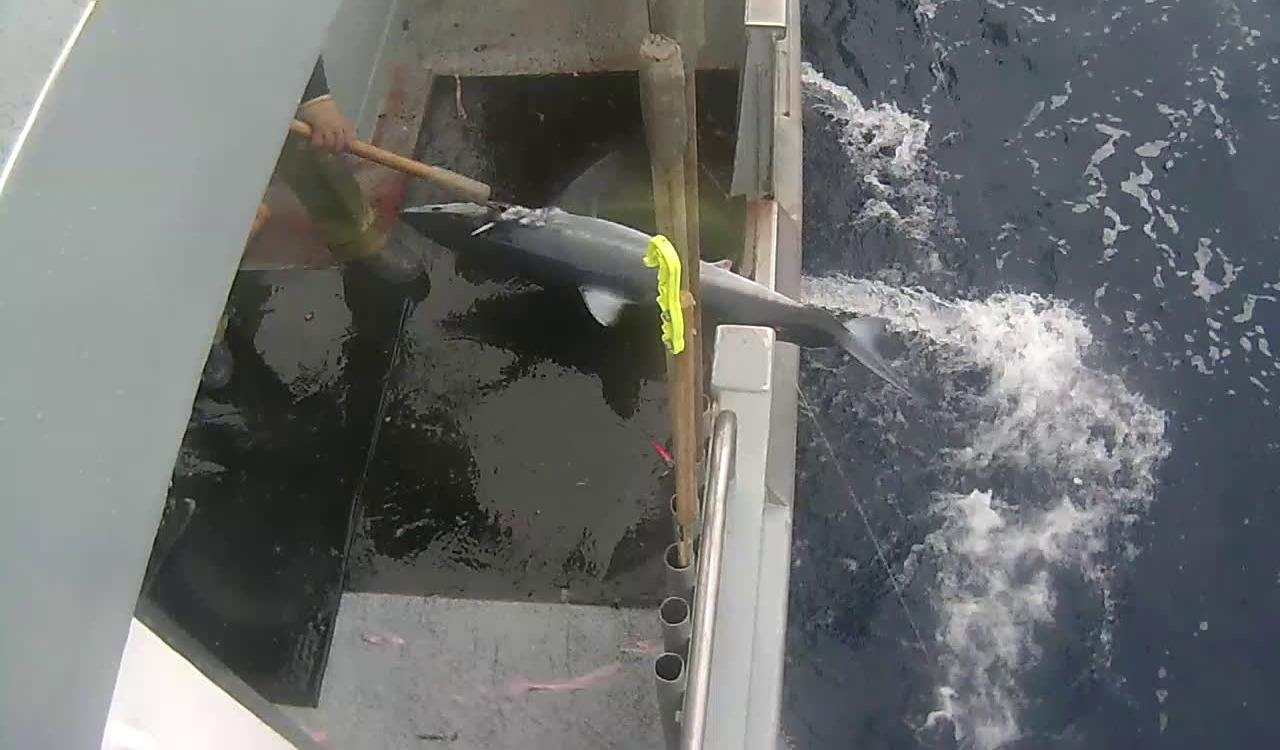
\includegraphics[width=8cm,keepaspectratio]{Images/colorpicture.jpg}
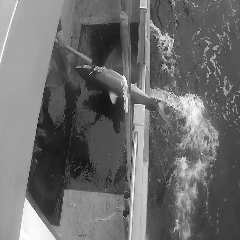
\includegraphics[width=3cm,keepaspectratio]{Images/test2.png}
\caption{Example of image change. Left original, right greyed and squared version.}
\end{figure}

The fish images were resized to uniformy 20x20 resolution. These images were not as clean as would be required by PCA, but given
the limitations of the dataset they were the best that could be used. Again these images were all set to greyscale for the purposes of this.
\begin{figure}[h]
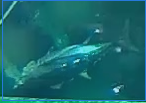
\includegraphics[width=2cm,keepaspectratio]{Images/fish1.png}
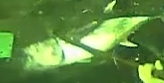
\includegraphics[width=2cm,keepaspectratio]{Images/fish2.png}
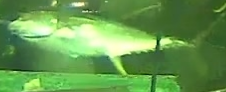
\includegraphics[width=2cm,keepaspectratio]{Images/fish3.png}
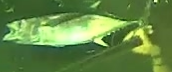
\includegraphics[width=2cm,keepaspectratio]{Images/fish4.png}
\caption{Example of original version of fish used.}
\end{figure}

In order to create an eigenspace the following code was used.
\begin{lstlisting}
k = 45
trial = 2

# load Data
path = "./HeadsAndTails/"
files = readdir(path)
n = 100
finalDim = (20,20)
fileInd = rand(1:size(files,1),n)
curfile = joinpath(path,files[1])
temp = convert(Array{Float64,2},convert(Image{Gray},load(curfile)))
temp = Images.imresize(temp,finalDim)
dim = size(temp)
D = zeros(prod(dim), n)
D[:,1] = vec(temp)
for i=2:n
    curfile = joinpath(path,files[fileInd[i]])
    temp = convert(Array{Float64,2},convert(Image{Gray},load(curfile)))
    temp = Images.imresize(temp,finalDim)
    D[:,i] = vec(temp)
end

# Normalize
x_bar = zeros(size(D,1),1)
for i =1:size(D,2)
    x_bar = x_bar + D[:,i]
end
x_bar = x_bar/size(D,2)

# Get residuals
X_tilde = D - repmat(x_bar ,1,size(D,2))

covm = X_tilde'*X_tilde
U, S, V = svd(covm)
Vk = zeros(size(V,1),k)
Vk = V[:,1:k]
Uk = X_tilde*Vk
norms = sqrt(diag(Uk'*Uk))

A = Uk./ repmat(norms',size(Uk,1),1)

# Project
Px = zeros(k,size(D,2))
for i=1:n
    Px[:,i] = A'*X_tilde[:,i]
end
;
\end{lstlisting}

The resulting eigenfish from this can be seen in figure 3.
\begin{figure}[h]

\includegraphics[width=1cm,keepaspectratio]{Images/eigfish1.png}
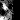
\includegraphics[width=1cm,keepaspectratio]{Images/eigfish2.png}

\includegraphics[width=1cm,keepaspectratio]{Images/eigfish3.png}
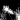
\includegraphics[width=1cm,keepaspectratio]{Images/eigfish4.png}
\caption{Top four eigenfish.}
\end{figure}

In order to do the sliding window the following code was used. This code takes the resolution, then
will travel by a 20x20 block to perform the projection. The threshold was set to 10 for this from experiments.

\begin{lstlisting}
function projtest(A,X,Px, threshold)
    p = A'*vec(X)
    n = size(Px,2)
    fish = false
    snorm = 0
    for i=1:n
        snorm+= norm(p-Px[:,i])
    end
    anorm = snorm/n
    if anorm <threshold
        return true
    else
        return false
    end
end

L = 240
w = 20
testOut = zeros(L,L)
for i in 1:w:L-w+1
    for j in 1:w:L-w+1
        sample = testim[i:i+w-1,j:j+w-1]
        fish = projtest(A,sample,Px,10)
        if fish
            testOut[i:i+w-1,j:j+w-1] = 1
        end
    end
end

grayim(testOut)
r = round(Int,prod(size(testOut)))
for i = 1:r
    if testOut[i] == 1
        testOut[i]=testim[i]
    end
end
grayim(testOut)
save("pca1.png",testOut)
\end{lstlisting}



The results of the PCA were disappointing. It seemed to prefer everything but the fish when
deciding if the part belonged to the final output or not. While the resulting image was sparse
there was no way to identify the fish from this anymore.

\begin{figure}[H]
\subfloat[]{
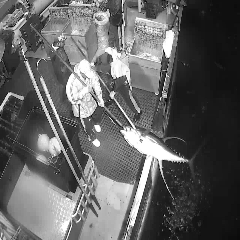
\includegraphics[width=3cm]{Images/test1.png}
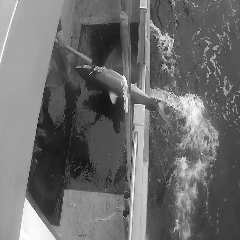
\includegraphics[width=3cm]{Images/test2.png}
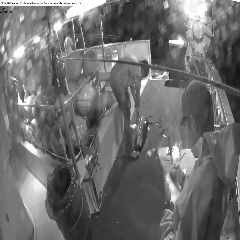
\includegraphics[width=3cm]{Images/test3.png}
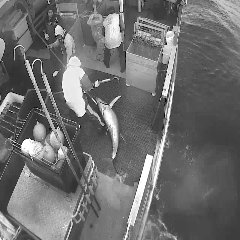
\includegraphics[width=3cm]{Images/test4.png}
}

\subfloat[]{
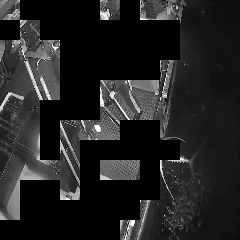
\includegraphics[width=3cm]{Images/pca1.png}
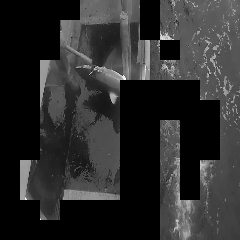
\includegraphics[width=3cm]{Images/pca2.png}
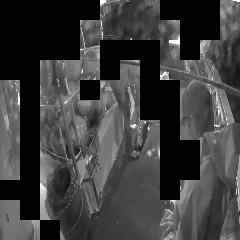
\includegraphics[width=3cm]{Images/pca3.png}
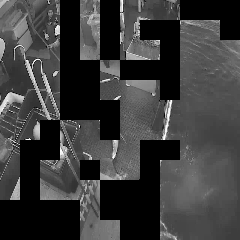
\includegraphics[width=3cm]{Images/pca4.png}
}
\caption{Original on top, PCA output on bottom}
\end{figure}


\subsection{Sparse Approximation}

\begin{lstlisting}
testim = convert(Array{Float64,2},Images.imresize(convert(Image{Gray},load("./Test/test7.jpg")), (220,220)))
Y = testim
X = Variable(size(testim))
E = Variable(size(testim))
lam = 1/sqrt(maximum(size(Y)))

problem = minimize(lam*norm(vec(X),1)+nuclearnorm(E),X+E==Y)
solve!(problem)
\end{lstlisting}

As stated previously this code solves for
\[ (A_{0} ,E_{0}) = argmin \ \norm{A}_{*} + \lambda \norm{E}_{1} \ subj A+E = Y \]
The output is shown below in figure 5.

\begin{figure}[H]
\subfloat[]{
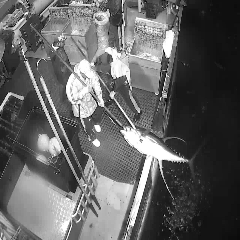
\includegraphics[width=3cm]{Images/test1.png}
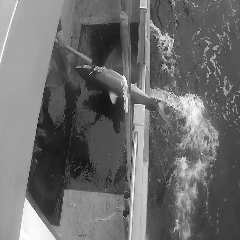
\includegraphics[width=3cm]{Images/test2.png}
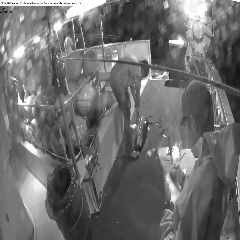
\includegraphics[width=3cm]{Images/test3.png}
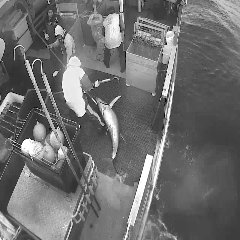
\includegraphics[width=3cm]{Images/test4.png}
}

\subfloat[]{
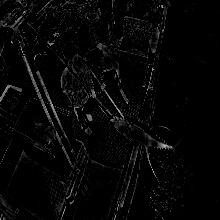
\includegraphics[width=3cm]{Images/sprs1.png}
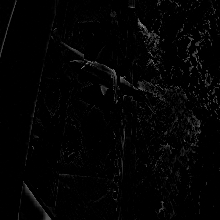
\includegraphics[width=3cm]{Images/sprs2.png}
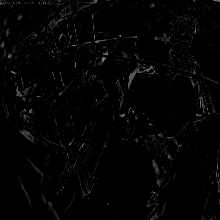
\includegraphics[width=3cm]{Images/sprs3.png}
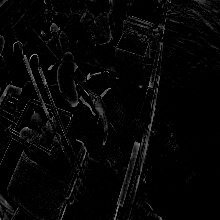
\includegraphics[width=3cm]{Images/sprs4.png}
}
\caption{Original on top, Sparse Approximation output on bottom}
\end{figure}

A few obvious things are that the image is much more sparse than the resulting one from PCA. Also, the fish
has also been outlined which is much improved from PCA. A close up is shown below.
\begin{figure}[H]
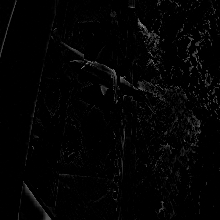
\includegraphics[width=7cm]{Images/sprs2.png}
\caption{Larger version of sparse output}
\end{figure}
The features of the fish are fully present in this image, and it was able to reduce the clutter of the image much
more than PCA.

\section{Conclusions}
A comparison on the effectiveness of PCA using sliding window technique, versus Sparse Matrix representation was used.
This was done in order to find objects within a cluttered image. What was found was the PCA performed poorly in its ability to find
the object that was given to it relative to the Sparse Matrix. However, PCA was much quicker, but being able to quickly get to the
incorrect answer does not make up for the limitations it comes to. In general, PCA requires much more time spent before the analysis to
clean up the image, while a sparse matrix can be formed without any priot knowledge of the structure.


\end{document}
